% ===============================================================================================
% ===============================================================================================
% PARALLELISM BASICS
%
% - Flynn
% - Amdahl's law
% - Gustaffson's law
% - speedup, etc..
% - Roofline model
%
% ===============================================================================================
% ===============================================================================================
\subsection{Parallelism basics}


\begin{frame}[containsverbatim]
\frametitle{Parallel computer}
\begin{center}
        {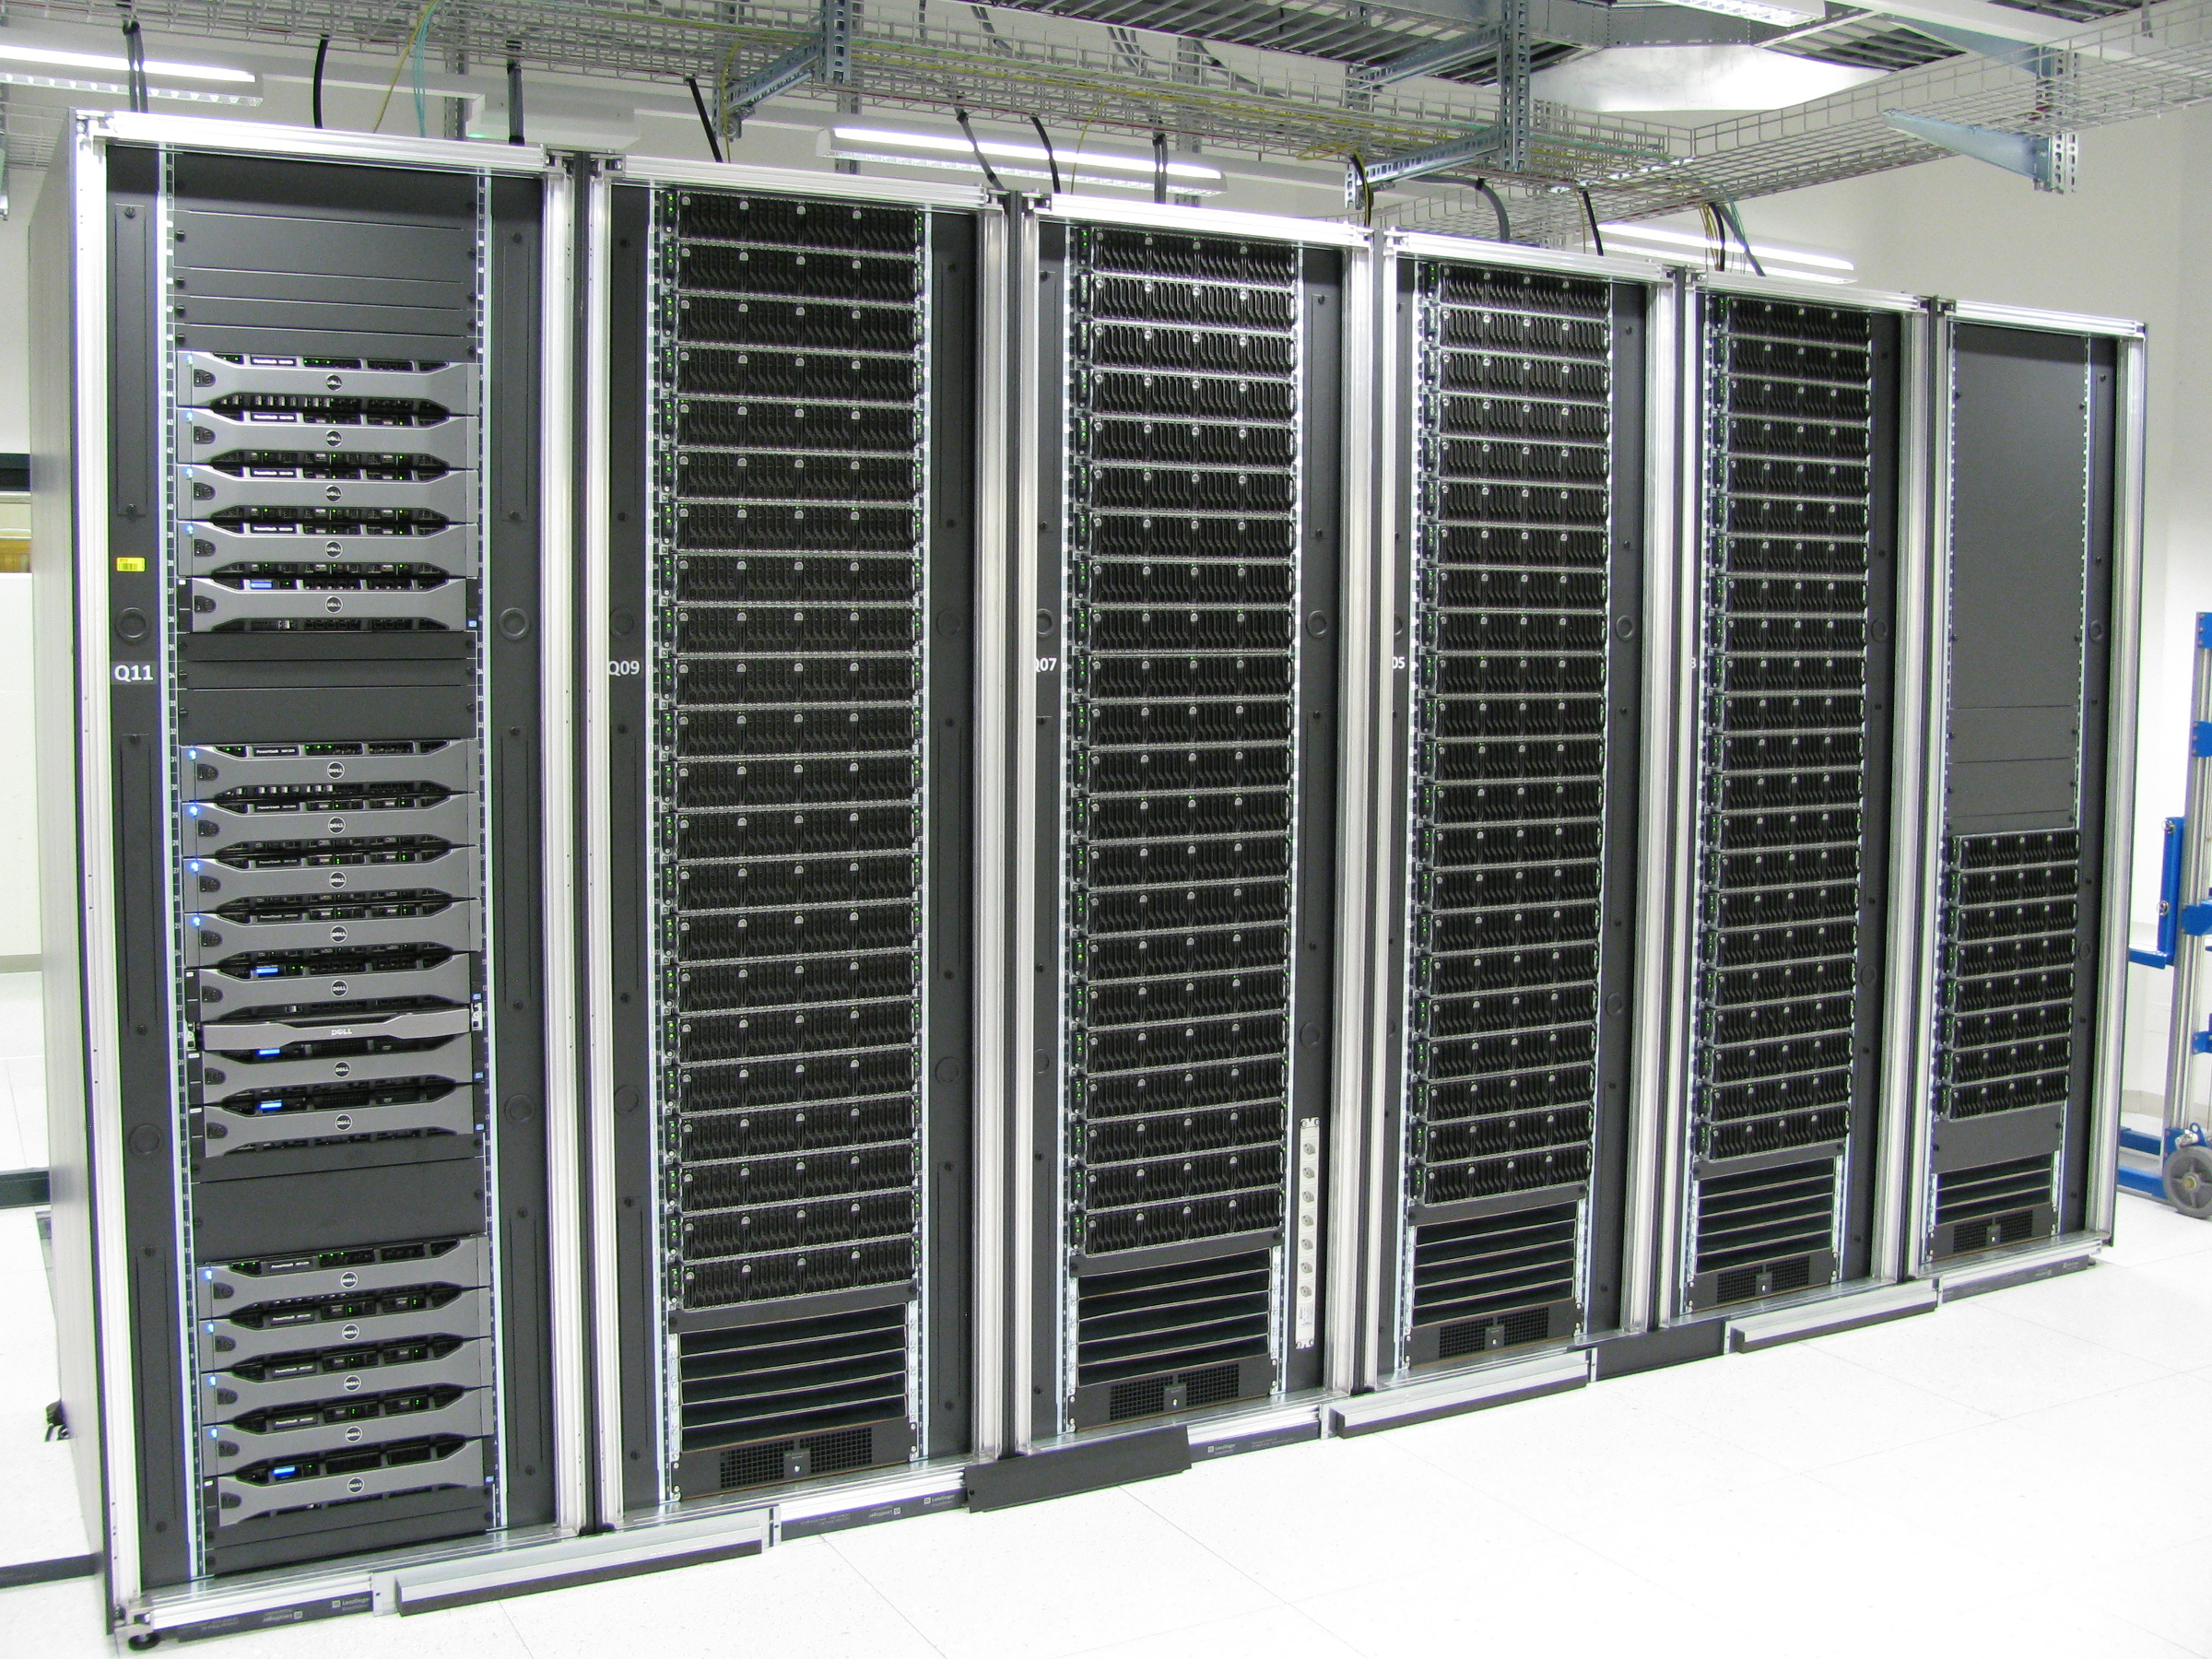
\includegraphics[height=7cm]{Day0/images/bellatrix2.jpg}}
\end{center}
\end{frame}

\begin{frame}[containsverbatim]
\frametitle{Parallel computer (cluster) HW components}
\begin{itemize}
	\item{\textbf{Nodes :} composed of
		\begin{itemize}
			\item{one or more \textbf{CPU} each with multiple \textbf{cores}}
			\item{\textbf{shared memory among the cores}}
			\item{\textbf{a NIC} (Networking Interface Card)}
		\end{itemize}
	}
	\item{\textbf{Interconnection network}}
	\item{\textbf{one (or more) Frontend} to access the cluster remotely}
\end{itemize}
\end{frame}

\begin{frame}[containsverbatim]
\frametitle{Parallel computer (cluster) SW components}
\begin{itemize}
	\item{\textbf{A scheduler} in order to share the resources among multiple users}
	\item{\textbf{A basic software stack} with compilers, linkers and basic parallel libraries}
	\item{\textbf{An application stack} with specific ready-to-use scientific applications}
\end{itemize}
\end{frame}



\begin{frame}[containsverbatim]
\frametitle{Vocabulary}
\begin{itemize}
	\item{\textbf{parallel computing :} data and/or task parallelism}
	\item{\textbf{supercomputing :} use of the fastest and largest machines in the world EFFICIENTLY}
	\item{\textbf{high performance computing (HPC) :} buzzword}
\end{itemize}
\end{frame}



\begin{frame}[containsverbatim]
\frametitle{Flynn taxonomy (1966)}
\begin{center}
\begin{tabular}{ l | c | c | }
	& Single instruction & Multiple instructions \\
\hline
   Single data & SISD & MISD  \\
    & Sequential processing & n/a  \\
\hline
   Multiple data & SIMD & MIMD \\
    & vector processing & distributed processing \\
\hline
 \end{tabular}
\end{center}
\end{frame}

\begin{frame}[containsverbatim]
\frametitle{Flynn taxonomy : examples}
\begin{center}
\begin{tabular}{ l | l | l | }
	& Single instruction & Multiple instructions \\
\hline
   Single data & - one core & - very rare  \\
\hline
   Multiple data & - Intel AVX512 (vectorization) & - Clusters \\
    & - GPU & \\
\hline
 \end{tabular}
\end{center}
\end{frame}


\begin{frame}[containsverbatim]
\frametitle{Parallelism ?}
Decomposition
\begin{itemize}
	\item{\textbf{on the data :} DATA PARALLELISM (SIMD)}
	\item{\textbf{on the tasks :} TASK PARALLELISM (MISD, MIMD)}
\end{itemize}

... or a mix of both !

\end{frame}

\begin{frame}[containsverbatim]
\frametitle{Data parallelism}
\begin{itemize}
	\item{loop-level parallelism}
	\item{data is distributed}
	\item{data resides on a global memory address space}
\end{itemize}
\end{frame}

\begin{frame}[containsverbatim]
\frametitle{Task parallelism}
\begin{itemize}
	\item{pipelining}
	\item{like an assembly chain}
	\item{a task is divided into a sequence of smaller tasks}
	\item{each task is executed on a specialized piece of hardware}
	\item{concurrently}
\end{itemize}
\end{frame}

\begin{frame}[containsverbatim]
\frametitle{Back to HPL (High Performance Linpack)}
\begin{itemize}
	\item{Remainder : solves $A x = b$ using Gauss partial pivoting}
	\item{We ran it on one node, but what about if we distribute the matrix A (and $x$ and $b$) over $p$ nodes ?}
	\item{Needs for a \textit{Message Passing API}. Choice is \textbf{MPI} (Message Passing Interface)}
	\item{HPL is used to rate supercomputers worldwide}
	\item{TOP500}
\end{itemize}
\end{frame}

\begin{frame}[containsverbatim]
\frametitle{HPL : parallel algorithm}
\begin{itemize}
	\item{Solves $A x = b$, where  $A \in \mathbb{R}^{n \times n}$ and $x,b \in \mathbb{R}^n$}
	\item{by computing LU factorization with row partial pivoting of the $n$ by $n+1$ coefficient matrix $[A,b]$ : $P_r[A,b] = [[L \cdot U],y]$, where $P_r,L,U \in \mathbb{R}^{n \times n}$ and $y \in \mathbb{R}^n$}
	\item{Finally : $U x = y$}
\end{itemize}
The data is ditributed onto a 2D grid (of dimension $P\times Q$) of processes using a block-cyclic scheme :
\begin{center}
\begin{tabular}{| p{0.5cm} | p{0.5cm} | p{0.5cm} | p{0.5cm} |}
\hline
$P_0$ & $P_1$ & $P_0$ & $P_1$ \\
\hline
$P_2$ & $P_3$ & $P_2$ & $P_3$ \\
\hline
$P_0$ & $P_1$ & $P_0$ & $P_1$ \\
\hline
$P_2$ & $P_3$ & $P_2$ & $P_3$ \\
\hline
\end{tabular}
\end{center}
\end{frame}




\begin{frame}[containsverbatim]
\frametitle{TOP500}
\begin{center}
        {
\includegraphics[height=5cm]{Day0/images/Top500_logo.png}}
\end{center}
\end{frame}


\begin{frame}[containsverbatim]
\frametitle{TOP500 : current list (November 2019)}
\scriptsize
\begin{tabular}{| l | l | l | l | l | l | l | }
\hline
 \textbf{Rank} & \textbf{Machine} & \textbf{\# cores} & \textbf{$R_{\infty}$} & \textbf{$R_{max}$} & \textbf{Power} & \textbf{Country}\\
               &                  &                   &  in TFlop/s           & in TFlop/s         & in KW & \\
\hline
\hline
1 & Summit & 2,414,592&148,600.0 &200,794.9 & 10,096 & USA\\
\hline
2 & Sierra & 1,572,480 &94,640.0 &125,712.0 & 7,438 & USA\\
\hline
3 & Sunway & 10,649,600 &93,014.6 &125,435.9 &15,371 & China\\
 & TaihuLight &  & & & &\\
\hline
4 & Tianhe-2A & 4,981,760 &61,444.5 & 100,678.7 &18,482 & China\\
\hline
5 & Frontera & 448,448 &23,516.4 &38,745.9 &n/a& USA\\
\hline
6 &  Piz Daint & 387,872 &21,230.0 &27,154.3 &2,384& Switzerland\\
\hline
7 &  Trinity & 979,072 &20,158.7 &41,461.2 &7,578& USA\\
\hline
8 &  Al Bridging & 391,680 &19,880.0 &32,576.6 &1,649& Japan\\
\hline
9 &  SuperMUC & 305,856 &19,476.6 &26,873.9 &n/a& Germany\\
\hline
10 & Lassen & 288,288 &18,200.0 &23,047.2 &n/a& USA\\
\hline

\end{tabular}
\end{frame}




%\begin{frame}[containsverbatim]
%\frametitle{TOP500 : current list (June 2018)}
%\scriptsize
%\begin{tabular}{| l | l | l | l | l | l | }
%\hline
% \textbf{Rank} & \textbf{Machine} & \textbf{\# cores} & \textbf{$R_{\infty}$} & \textbf{$R_{max}$} & \textbf{Power} \\
%               &                  &                   &  in TFlop/s           & in TFlop/s         & in KW \\
%\hline
%\hline
%1 & Summit & 2,282,544&122,300.0 &187,659.3 & 8,806 \\
%\hline
%2 & Sunway TaihuLight & 10,649,600 &93,014.6 &125,435.9 &15,371 \\
%\hline
%3 & Sierra & 1,572,480 &71,610.0 &119,193.6 & n/a \\
%\hline
%4 & Tianhe-2A & 4,981,760 &61,444.5 & 100,678.7 &18,482 \\
%\hline
%5 &  Al Bridging & 391,680 &19,880.0 &32,576.6 &1,649\\
%\hline
%6 &  Piz Daint & 361,760 &19,590.0 &25,326.3 &2,272\\
%\hline
%7 &  Titan & 560,640 &17,590.0 &27,112.5 &8,209\\
%\hline
%8 &  Sequoia & 1,572,864 &17,173.2 &20,132.7 &7,890\\
%\hline
%9 &  Trinity & 979,968 &14,137.3 &43,902.6 &3,844\\
%\hline
%10 &  Cori & 622,336 &14,014.7 &27,880.7 &3,939\\
%\hline
%
%\end{tabular}
%\end{frame}





% ===============================================================================================
% ===============================================================================================
% PARALLEL APPLICATIONS AND ALGORITHMS
%
%
% ===============================================================================================
% ===============================================================================================
\subsection{Parallel applications and algorithms}

\begin{frame}[containsverbatim]
\frametitle{}

\begin{center}
\textbf{Theoretical analysis of a code}
\end{center}

\end{frame}


\begin{frame}[containsverbatim]
\frametitle{Performance analysis}
\textbf{Before starting parallelization : insight of the application} 
\begin{itemize}
	\item{is the algorithm/application a good candidate for parallelization ?}
	\item{Which parallelization strategy should I choose ?}
	\item{How should I partition the problem ?}
\end{itemize}
\textbf{Helps understanding and improving existing implementations}
\begin{itemize}
	\item{do the benchmark match the performance predictions ?}
	\item{which factors have most influence on the performance ?}
	\item{which HW fits most to the applications needs ?}
\end{itemize}
\end{frame}




\begin{frame}
\frametitle{Speedup and efficiency}

\[
S(p) = \frac{T_{1}}{T_{p}} \qquad E(p) = \frac{S(p)}{p}
\]

where

\begin{itemize}
	\item{\textbf{$T_1$ :} Execution time using 1 process }
	\item{\textbf{$T_p$ :} Execution time using p process }
	\item{\textbf{$S(p)$ :} Speedup of $p$ processes }
	\item{\textbf{$E(p)$ :} Parallel Efficiency }
\end{itemize}

Example :

\begin{columns}
    \begin{column}{0.47\textwidth}
\begin{tabular}{| l | l | l | l |}
\hline
 \textbf{n} & \textbf{Walltime in [s]} & \textbf{S(p)}& \textbf{E(p)} \\
\hline
\hline
1 & 24.5 & 1.0 & 1.0\\
\hline
2 & 13.4 & 1.8 & 0.9\\
\hline
4 & 6.8 & 3.6 & 0.9\\
\hline
8 & 4.0.5 & 6.1 & 0.76\\
\hline
\end{tabular}
    \end{column}
    \begin{column}{0.5\textwidth}
        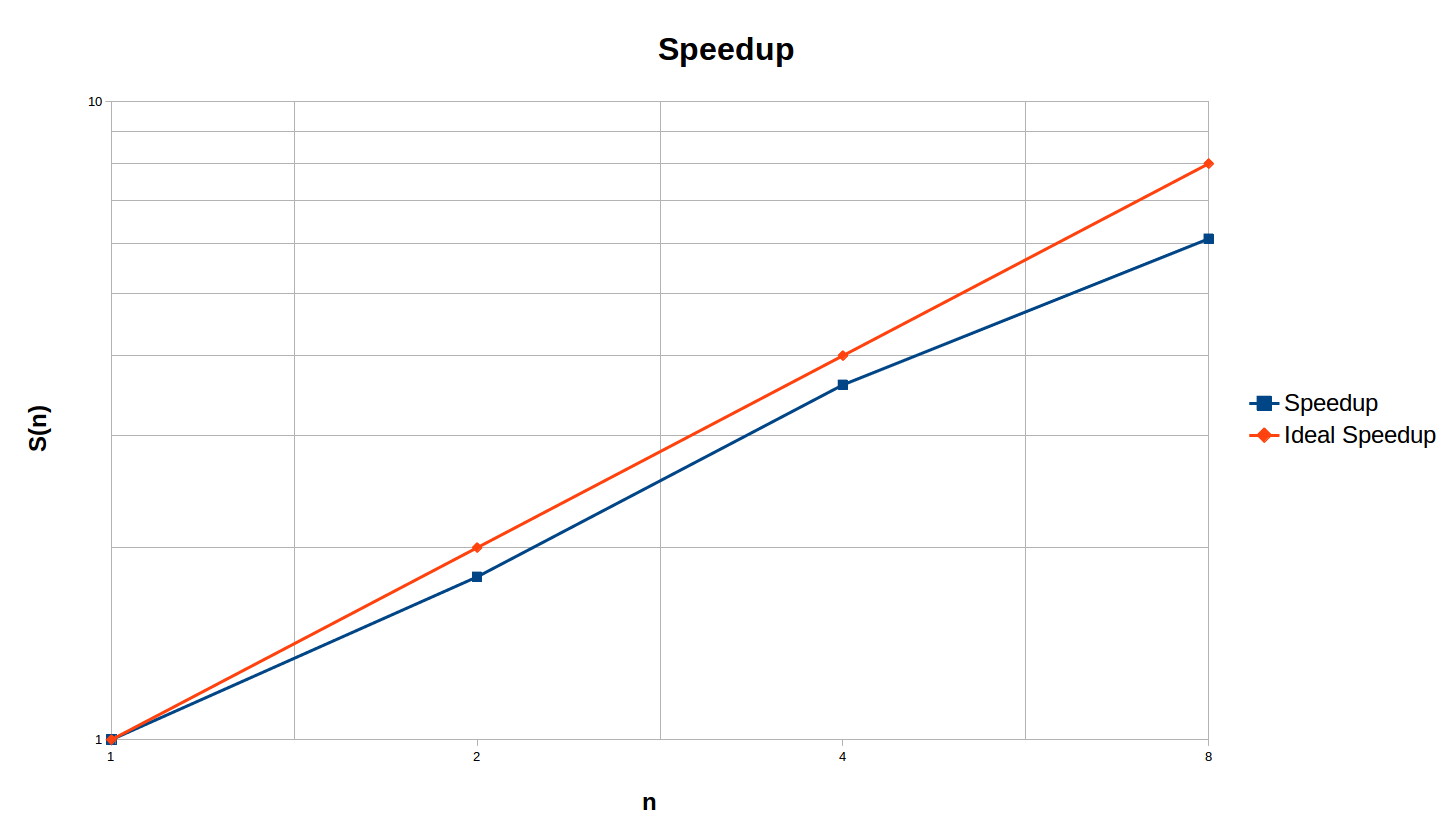
\includegraphics[width=\textwidth]{Day0/images/speedup.png} 
    \end{column}
\end{columns}
\end{frame}

\begin{frame}[containsverbatim]
\frametitle{Amdahl's law}
\begin{itemize}
	\item{\textbf{Maximum achievable speedup} for an application where a fraction $f$ cannot be parallelized}
	\item{$S(p)  \leqslant  \frac{1}{f + \frac{(1-f)}{p}}$}
	\item{or $S(p)  \leqslant  \frac{p}{1 + (p-1) \cdot f}$}
	\item{$S(p)$ is always lower than $\frac{1}{f}$: $lim_{p \rightarrow \infty} S(p)  \leqslant \frac{1}{f}$}
	\item{Desirable : $f < \frac{1}{p}$}
	\item{provides an upperbound}
\end{itemize}
\end{frame}

\begin{frame}[containsverbatim]
\frametitle{Amdahl's law}
\begin{center}
        {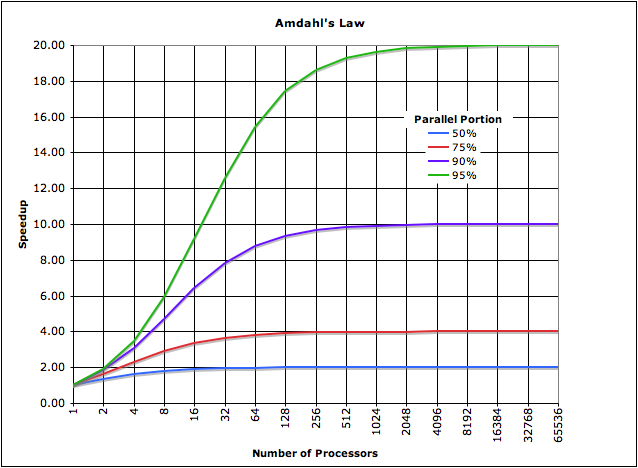
\includegraphics[height=5cm]{Day0/images/amdahl.png}}
\end{center}
\end{frame}


\begin{frame}[containsverbatim]
\frametitle{Amdahl's law (deduce $f$)}
\begin{align} 
S_p &= \frac{1}{f + \frac{(1-f)}{p}}
\end{align}
then 
\begin{align} 
S_p \cdot f + \frac{S_p}{p} - S_p \cdot \frac{f}{p} &= 1 
\end{align}
finally :
\begin{align} 
f &= \frac{1 - \frac{S_p}{p}}{S_p - \frac{S_p}{p}} = \frac{\frac{1}{S_p} - \frac{1}{p}}{1 - \frac{1}{p}}
\end{align}
$f$ comprise communication overhead
\end{frame}

\begin{frame}
\frametitle{Amdahl and Gustafson}
\begin{exampleblock}{Observation}
Amdahl's law is an estimation for a \textbf{fixed problem size} $n$.
\end{exampleblock}
\begin{alertblock}{Problem}
If we increase the problem size, the relative sequential part can be made smaller and smaller \textit{if it is of lower complexity than the parallel part of the problem}
\end{alertblock}
\begin{alertblock}{Solution}
Take the problem size $n$ into account. This is Gustafson's law (or Gustafson's complement to Amdahl's law)
\end{alertblock}
\end{frame}


\begin{frame}[containsverbatim]
\frametitle{Gustafson's law}
$s$ is the sequential portion, $a$ is the parallel portion. The sequential ($t_s$) and parallel ($t_p$) are:

\[
t_s = s + a \cdot n \qquad t_p = s + a \cdot \frac{n}{p}
\]

then the Speedup $S_p$ is :

\begin{align} 
S_p &= \frac{t_s}{t_p} = \frac{s + a \cdot n}{s + a \cdot \frac{n}{p}} = \frac{\frac{s}{n} + a}{\frac{s}{n} + \frac{a}{p}}
\end{align}

Note $lim_{n \rightarrow \infty} S_p = p$

\end{frame}




\begin{frame}[containsverbatim]
\frametitle{Gustafson's law}
\begin{center}
        {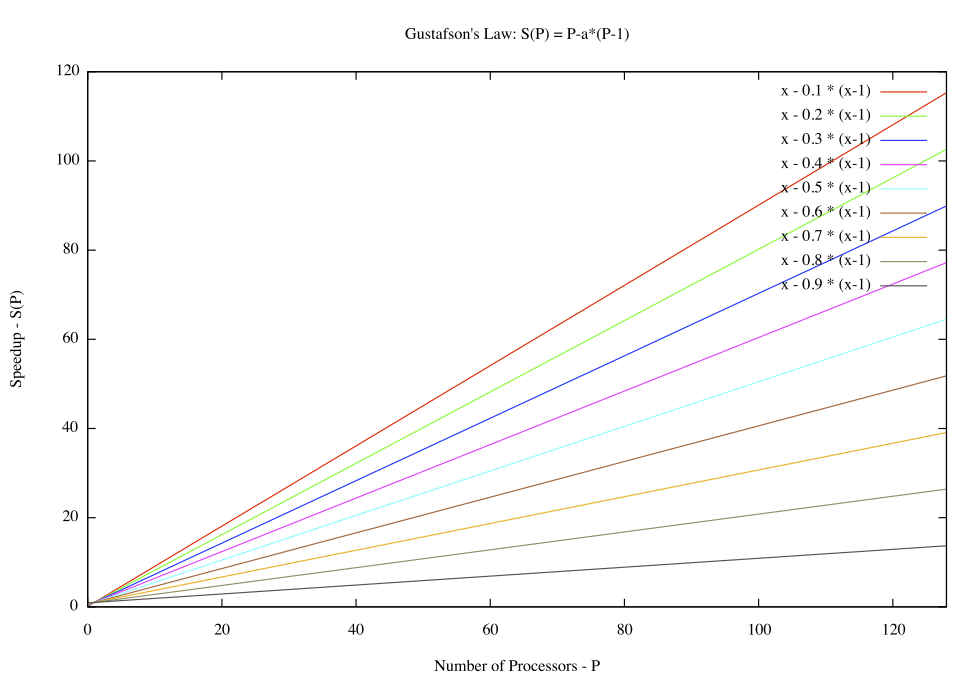
\includegraphics[height=5cm]{Day0/images/gustafson.png}}
\end{center}
\end{frame}

\begin{frame}[containsverbatim]
\frametitle{Complexity analysis}
\begin{exampleblock}{Observation}
The speedup $S(p)$ is determined by the \textbf{computation time} and the \textbf{communication time}, function of the problem size $n$
\end{exampleblock}
\begin{exampleblock}{Communication \& computation time}
It is an overhead to the parallel execution time. It can be partially hidden by computation.
\end{exampleblock}
\begin{exampleblock}{Complexity}
Computing the \textbf{complexity} $\mathcal{O}(n,p)$ provides an insight into the parallelization potential.
\end{exampleblock}
\end{frame}

%%%%%%%%%%%%%%%%%%%%%%%%%%%%%%%%%%%%%%%%%%%%%%%%%%%%%%%%
%%%%%%%%%%%%%%%%%%%%%%%%%%%%%%%%%%%%%%%%%%%%%%%%%%%%%%%%
% FIXME : Prendre l'exemple du matrice vecteur à la place de matrice matrice
% voir page 9 : https://www3.nd.edu/~zxu2/acms60212-40212-S12/Lec-05.pdf
% plus : http://www.hpcc.unn.ru/mskurs/ENG/DOC/pp07.pdf (complexity analysis + dependencies)
%%%%%%%%%%%%%%%%%%%%%%%%%%%%%%%%%%%%%%%%%%%%%%%%%%%%%%%%
%%%%%%%%%%%%%%%%%%%%%%%%%%%%%%%%%%%%%%%%%%%%%%%%%%%%%%%%


\begin{frame}[containsverbatim]
\frametitle{Complexity analysis : example $c = A \cdot b$}
\textbf{Full $N \times N $ matrix vector multiplication with the naïve method $\mathcal{O}(N^2)$}
\begin{lstlisting}[language=C,frame=lines]
   struct timeval t;
   double t1 = gettimeoftheday(&t,0);
   for (i=0;i<N;i++){
      for (j=0;j<N;j++){
         c[i] = c[i] + A[i][j]*b[j];
      }
   }
   double t2 = gettimeoftheday(&t,0);
   double mflops = 2.*(double)N*(double)N / (t2-t1) / 1.0E6;
\end{lstlisting}
\end{frame}


\begin{frame}[containsverbatim]
\frametitle{Complexity analysis : example $c = A \cdot b$}
\textbf{Sequential algorithm :}
\begin{itemize}
	\item{\textbf{Time complexity :} $\mathcal{O}(N)$}
	\item{\textbf{Size complexity :} $\mathcal{O}(N^2)$}
\end{itemize}
\end{frame}

\begin{frame}[containsverbatim]
\frametitle{Complexity analysis : example $c = A \cdot b$}
\textbf{Parallel version}
\begin{lstlisting}[language=C,frame=lines]
   t1 = MPI_Wtime();
   MPI_Bcast(b, ndiag, MPI_FLOAT, 0, MPI_COMM_WORLD);
   MPI_Scatter(A,(nn_loc*ndiag),MPI_FLOAT,A_loc,(nn_loc*ndiag),MPI_FLOAT,0,MPI_COMM_WORLD);
   t2 = MPI_Wtime();		
   for (j=0;j<ndiag;j++){
      for (i=0;i<nn_loc;i++){
         c[i] = c[i] + A_loc[i+j*nn_loc]*b[i];
      }
   }
   t3 = MPI_Wtime();
   MPI_Gather(c,nn_loc,MPI_FLOAT,b,nn_loc,MPI_FLOAT,0,MPI_COMM_WORLD);
   t4 = MPI_Wtime();
\end{lstlisting}
\end{frame}


%\begin{frame}[containsverbatim]
%\frametitle{Complexity analysis : example $c = A \cdot b$}
%\textbf{Parallel version}
%\begin{lstlisting}[language=C,frame=lines]
%   t1 = MPI_Wtime();
%   MPI_Bcast(U, ndiag, MPI_FLOAT, 0, MPI_COMM_WORLD);
%   MPI_Scatter(A,(nn_loc*ndiag),MPI_FLOAT,A_loc,(nn_loc*ndiag),MPI_FLOAT,0,MPI_COMM_WORLD);
%   t2 = MPI_Wtime();		
%   for (j=0;j<ndiag;j++){
%      for (i=0;i<nn_loc;i++){
%         Ua[i] = Ua[i] + A_loc[i+j*nn_loc]*U[i];
%      }
%   }
%   t3 = MPI_Wtime();
%   MPI_Gather(Ua,nn_loc,MPI_FLOAT,U,nn_loc,MPI_FLOAT,0,MPI_COMM_WORLD);
%   t4 = MPI_Wtime();
%\end{lstlisting}
%\end{frame}



\begin{frame}[containsverbatim]
\frametitle{Complexity analysis : example $c = A \cdot b$}
\textbf{Parallel algorithm over $p$ processes:}
\begin{itemize}
	\item{\textbf{Computational complexity :} $\mathcal{O}(\frac{N^2}{p})$}
	\item{\textbf{Communication complexity :} $\mathcal{O}(log p + N)$}
	\item{\textbf{Overall complexity :} $\mathcal{O}(\frac{N^2}{p} + log p + N)$}
	\item{for \textit{reasonably} large $N$, latency is neglictible compared to bandwidth}
	\item{The algorithm is not scalable}
\end{itemize}
\end{frame}







\begin{frame}[containsverbatim]
\frametitle{On the importance of algorithmic analysis}
\textbf{Full $N \times N $ matrix matrix multiplication with the naïve method $\mathcal{O}(N^3)$}
\begin{lstlisting}[language=C,frame=lines]
   struct timeval t;
   double t1 = gettimeoftheday(&t,0);
      for (i=0;i<N;i++){
         for (j=0;j<N;j++){
            for (k=0;k<N;k++){
               C[i][j]=C[i][j] + A[i][k]*B[k][j];
            }
         }
      }
   double t2 = gettimeoftheday(&t,0);
   double mflops = 2.0*pow(N,3) / (t2-t1) / 1.0E6 ;
\end{lstlisting}
\end{frame}

\begin{frame}[containsverbatim]
\frametitle{On the importance of algorithmic analysis}
\begin{center}
        {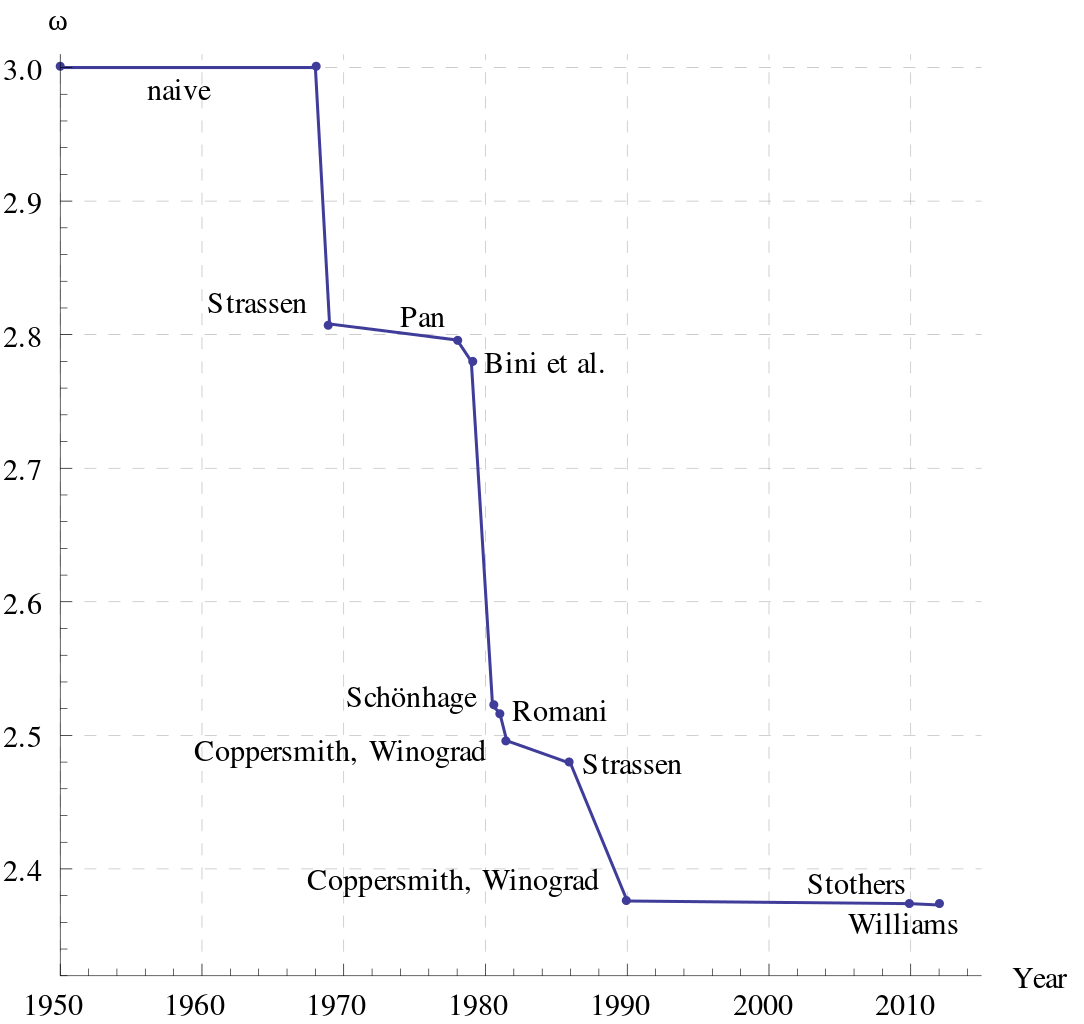
\includegraphics[height=5cm]{Day0/images/dgemm-complexity.png}}
\end{center}
\end{frame}


%\begin{frame}[containsverbatim]
%\frametitle{Complexity analysis : HPL example}
%\begin{exampleblock}{Complexity}
%$\mathcal{O}(n^3)$ more specifically $\frac{2}{3} n^3 " 2 n^2 + \mathcal{O}(n)$ floating-point multiplications and additions 
%\end{exampleblock}
%
%\end{frame}




\begin{frame}[containsverbatim]
\frametitle{Task dependency graph}
\begin{center}
        {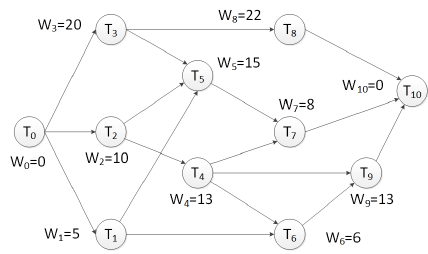
\includegraphics[height=3cm]{Day0/images/dependency.png}}
\end{center}
{\tiny Image from : Wu, Hao \& Hua, Xiayu \& Li, Zheng \& Ren, Shangping. \textit{Resource and Instance Hour Minimization for Deadline Constrained DAG Applications Using Computer Clouds}. IEEE TPDS. 2015}
\begin{itemize}
	\item{essentially a DAG (nodes = tasks, edges = dependencies)}
	\item{\textbf{critical path :} the longest path from starting task to the ending task}
	\item{\textbf{average degree of concurrency :} total amount of work devided by the critical path length}
\end{itemize}
\end{frame}




\begin{frame}[containsverbatim]
\frametitle{New bug in concurrent computing : deadlock}
\begin{center}
        {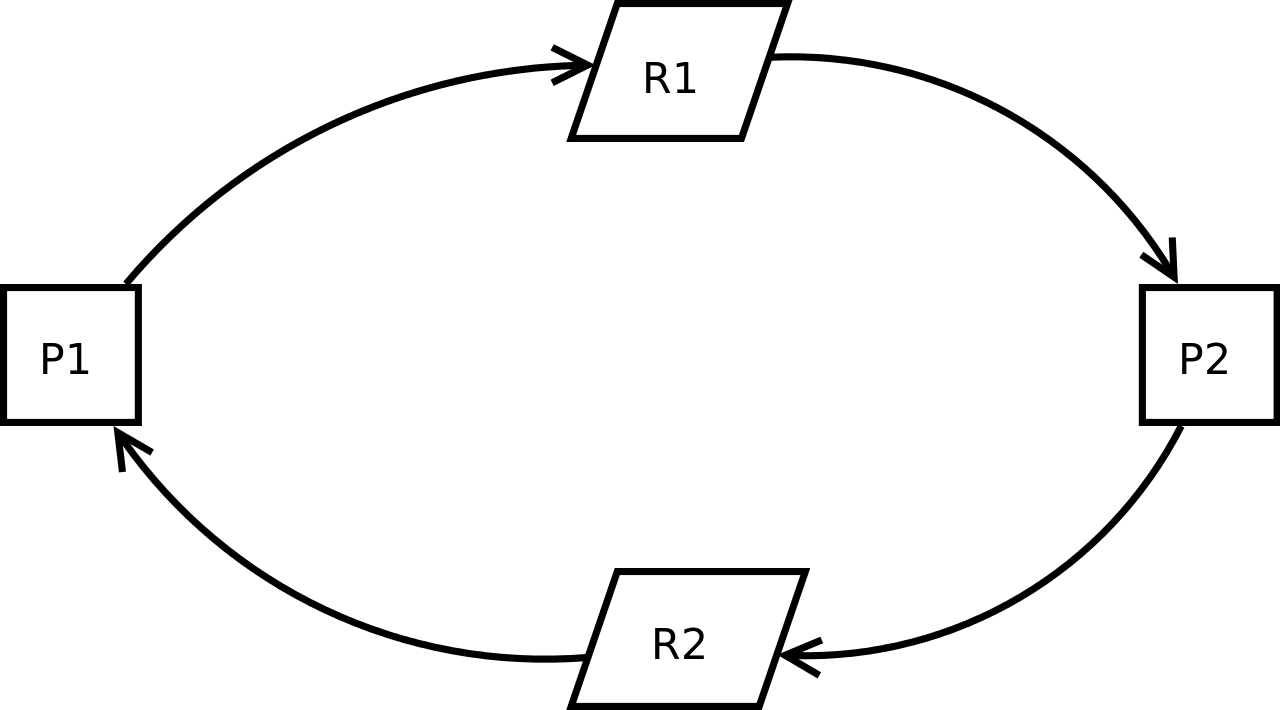
\includegraphics[height=3cm]{Day0/images/deadlock.png}}
\end{center}
\begin{itemize}
	\item{P1 holds resource R2 and requires R1}
	\item{P2 holds resource R1 and requires R2}
	\item{\textbf{deadlock !!}}
\end{itemize}
\end{frame}


\begin{frame}[containsverbatim]
\frametitle{New bug in concurrent computing : race condition}
\begin{itemize}
	\item{arise in concurrent computing when two (or more) processes depends on a sequence or timing on a shared variable}
	\item{example : $a = 0$ is a shared variable. P1 will do $a+1$ while P2 will do $a+2$ : 
		\begin{enumerate}
			\item{[P1] read $a = 0$}
			\item{[P2] read $a = 0$}
			\item{[P1] incr $a = 1$}
			\item{[P2] incr $a = 2$}
		\end{enumerate}
		}
	\item{The order can lead to different $a$ values : if 2 and 3 are interverted :
		\begin{enumerate}
			\item{[P1] read $a = 0$}
			\item{[P1] incr $a = 1$}
			\item{[P2] read $a = 1$}
			\item{[P2] incr $a = 3$}
		\end{enumerate}
	}
	\item{\textbf{race condition !!}}
\end{itemize}

\end{frame}





